\newpage

\subsection{Issuance Case Study} 

\noindent Bob decides to purchase 100 havvens at \$1 each. Consider the following initial conditions:

\begin{align*}
C_{max} &= 0.5 & C_{opt} &= 0.4 & C &= 0.4 \\
P_n &= 1 & P_h &= 1 & H_i &= 100 \\
\sigma &= 50 & \phi &= 3 & a&= 1.25
\end{align*}

\noindent The system is in price equilibrium, with the global collateralisation ratio $C$ equal to the optimal collateralisation ratio $C_{opt}$. Initially,  Bob's wallet contains only free havvens.

\begin{figure}[h!]
\centering
    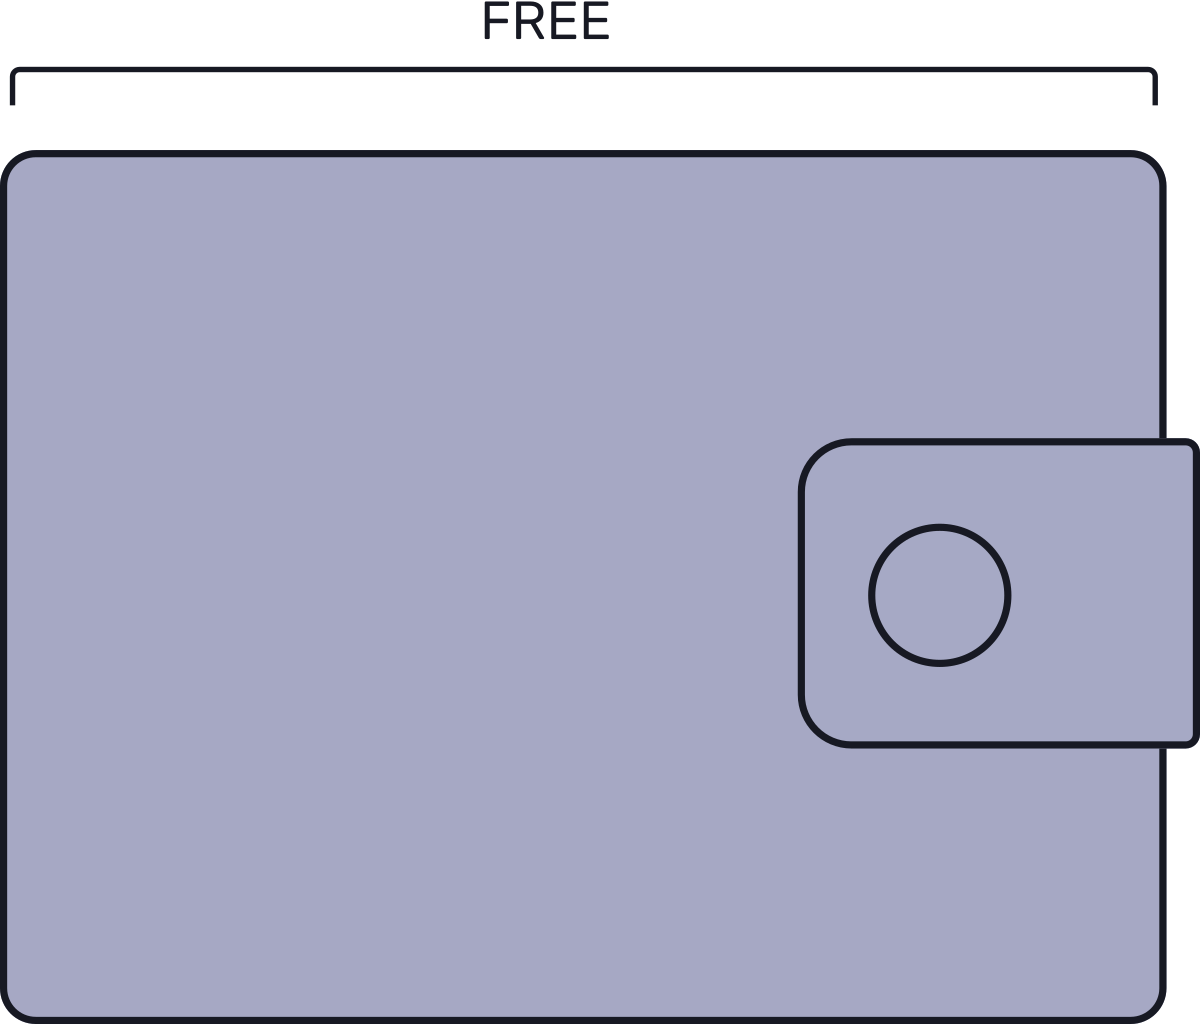
\includegraphics[width=0.40\textwidth]{img/wallet}
\end{figure}

\noindent Bob wants to earn the maximum possible fees, so he issues nomins up to $C_{opt}$. The system generates 40 nomins and escrows 80 of his havvens, locking \$80 worth of value in the system. The nomins are sold for \$40 worth of ether and the proceeds are transferred to Bob's account.
\begin{figure}[h!]
\centering
    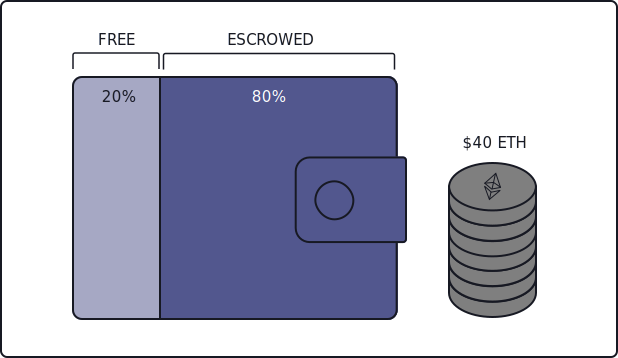
\includegraphics[width=0.6\textwidth]{img/escrowed}
\end{figure}

\noindent \textbf{Nomin Price Change} This example shows how the system incentivises havven holders to correct instability in the nomin price.

\begin{enumerate}
\item{As a consequence of reduced demand in decentralised trading markets, the nomin price $P_n$ drops to \$0.90. The system needs to incentivise havven holders to reduce the supply of nomins so that the price returns to \$1.00.}
\item{First, consider that both $C$ and Bob's $C_i$ have decreased to 0.36. Since the nomin price has changed, $C_{opt}$ is recalculated to 0.342, which is smaller than both $C_i$ and $C$. Consequently, $C_{max}$ also changes to 0.4275. This increases the percentage of Bob's havvens that are locked.}
\begin{figure}[h!]
\centering
    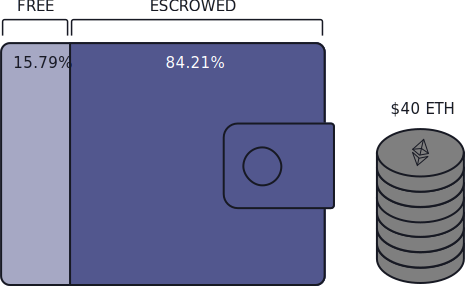
\includegraphics[width=0.6\textwidth]{img/pn_drop}
\end{figure}
\item{Bob now has a higher dollar value of locked havvens and his $C_i > C_{opt}$. This means that he is no longer receiving the maximum fee rate $\alpha_{base}$. In order to return to $\alpha_{base}$ he must lower his $C_i$ back to $C_{opt}$ by burning some nomins. He needs to work out how many to burn.}
\item{He should burn 2 nomins so that he has 38 total issued, which will cost \$1.80. When the system completes this process, his locked havvens will reduce back to 80. In addition, his $C_i$ is equal to $C_{opt}$ at 0.342, which means he is once again receiving the maximum fee rate.}
\begin{figure}[h!]
\centering
    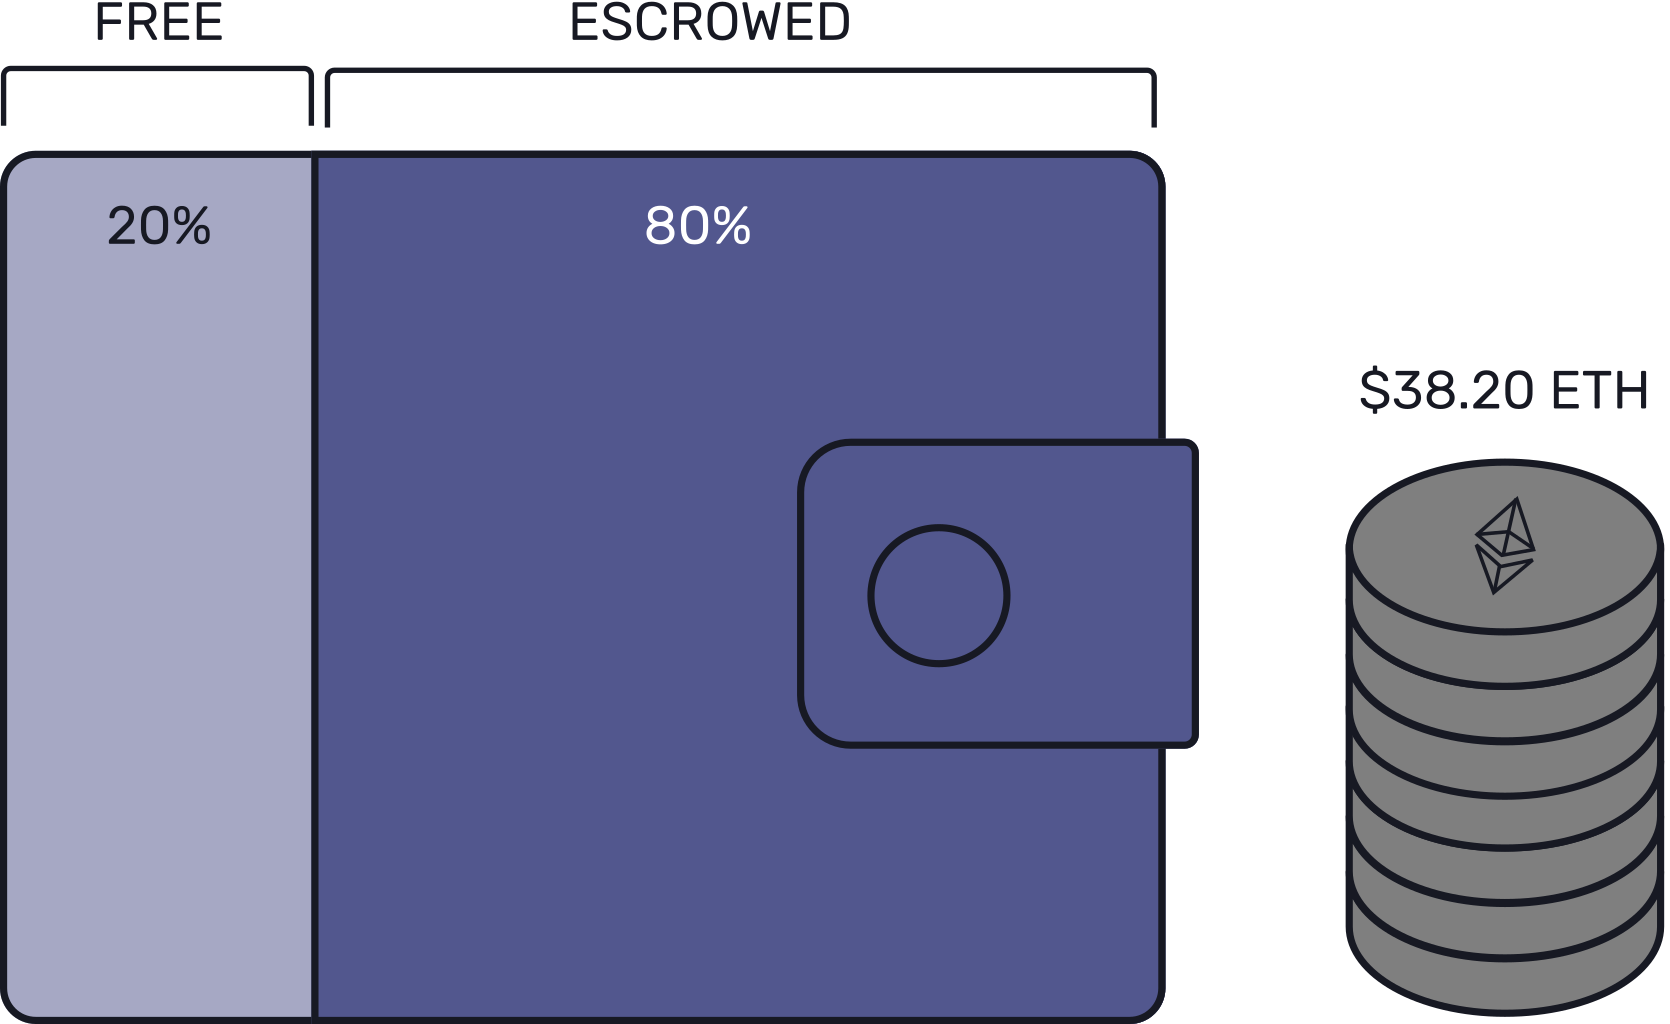
\includegraphics[width=0.6\textwidth]{img/post_burn}
\end{figure}
\item{Bob has taken the correct actions to raise the low nomin price. By electing to burn nomins, the system performed a limit buy order on his behalf, putting upward pressure on the nomin price. As compensation for doing so, he is rewarded with the optimal fee rate $\alpha_{base}$.}
\end{enumerate}

\newpage

\noindent \textbf{Havven Price Change (Market Price)} This example illustrates how the system maintains the dollar value of the underlying collateral by adjusting the quantity of a user's escrowed havvens when the havven price changes. Consider the same initial conditions as before:

\begin{align*}
C_{max} &= 0.5 & C_{opt} &= 0.4 & C &= 0.4 \\
P_n &= 1 & P_h &= 1 & H_i &= 100 \\
\sigma &= 50 & \phi &= 3 & a&= 1.25
\end{align*}

\begin{enumerate}
\item{Like before, Bob elects to issue up to $C_{opt}$ in order to maximise fees.}
\begin{figure}[h!]
    \centering
    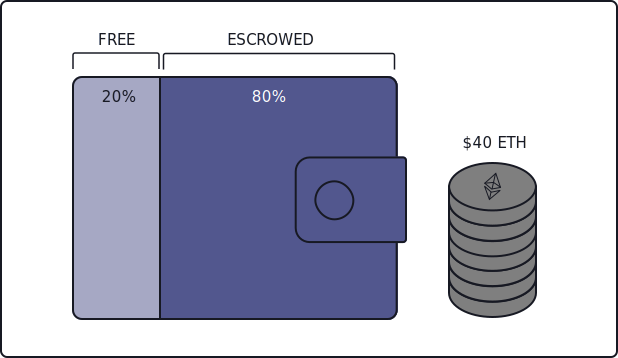
\includegraphics[width=0.6\textwidth]{img/escrowed}
\end{figure}
\item{The havven price $P_h$ drops to \$0.90, which means the value of Bob's wallet has decreased to \$90. Both $C$ and Bob's $C_i$ have increased to 0.44. Since the nomin price has not changed, the system does not need to incentivise issuance or burning. This is reflected in the new value of $C_{opt}$, which changes to 0.44, matching $C$ and $C_i$. }
\item{However, the system needs to escrow more of Bob's havvens to maintain the dollar value of the locked collateral. The system has now locked around 89\% of Bob's havvens, to maintain \$80 of locked collateral.}
\begin{figure}[h!]
    \centering
    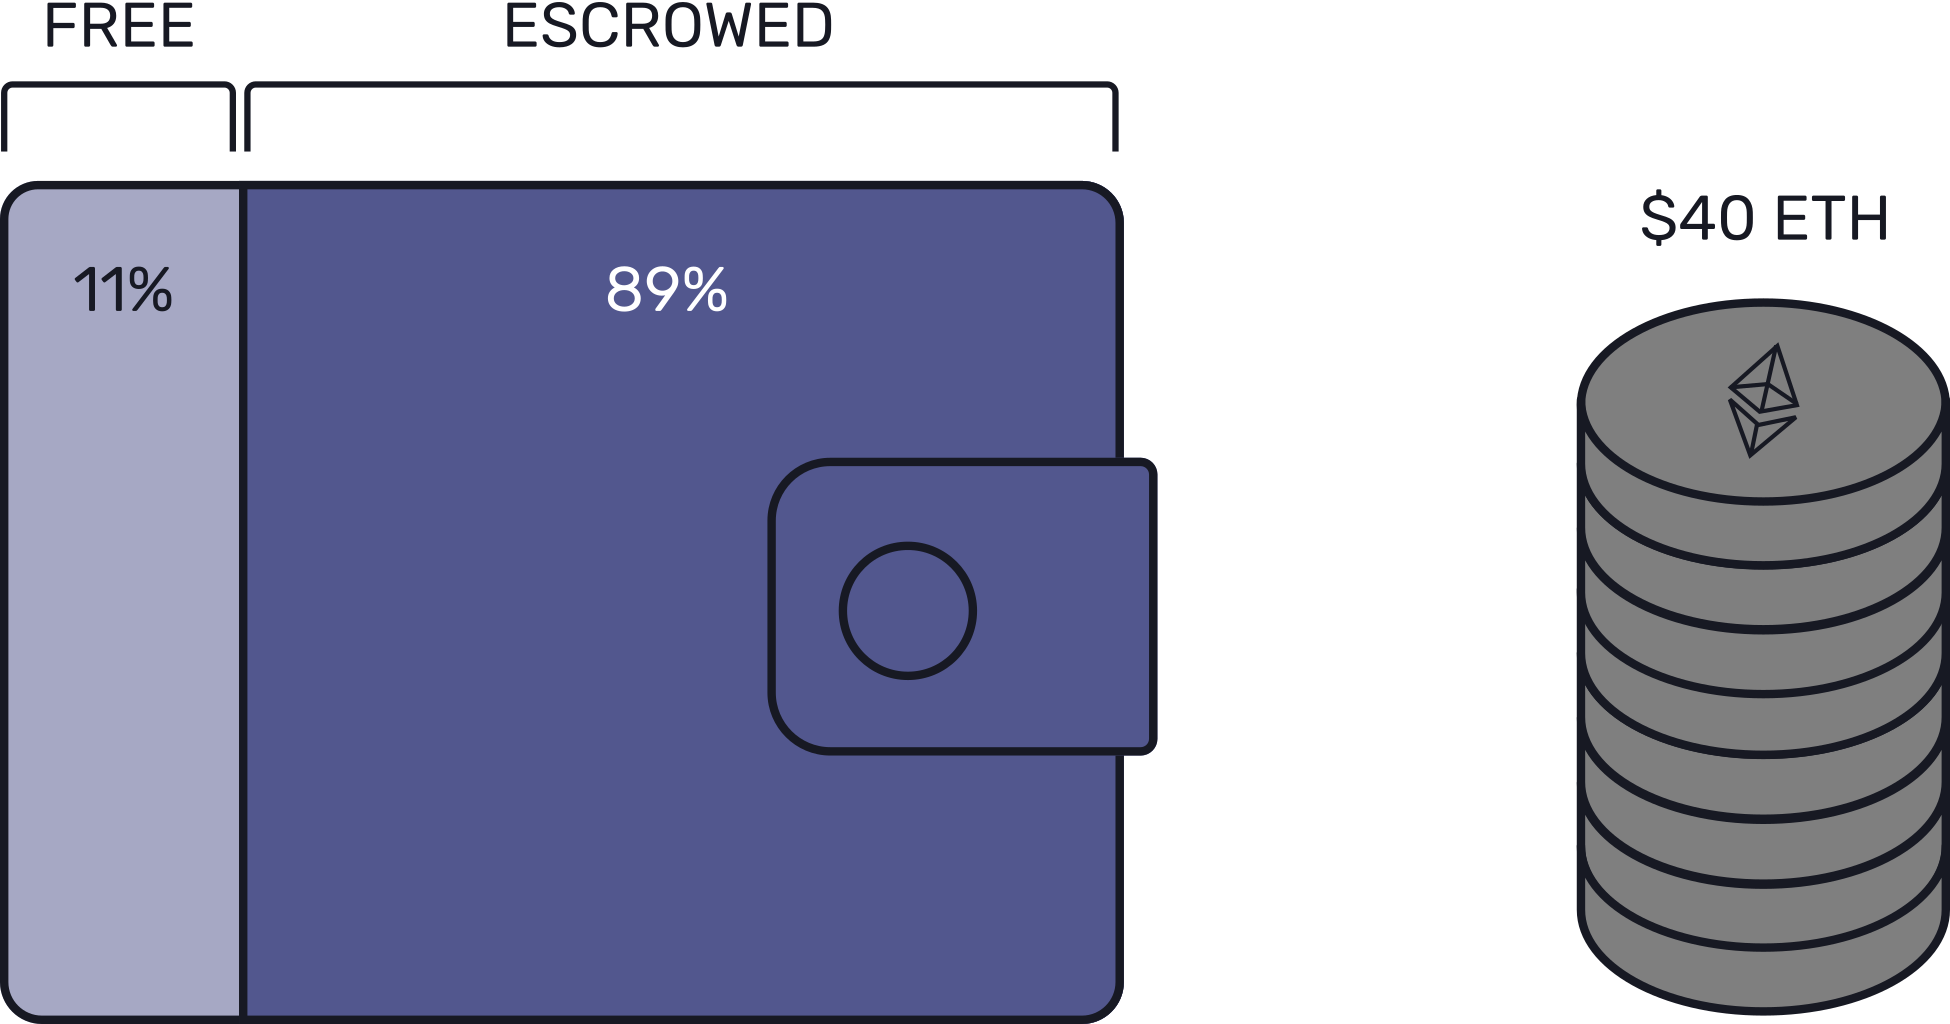
\includegraphics[width=0.6\textwidth]{img/ph_drop}
\end{figure}
\end{enumerate} 
